\documentclass[]{article}
\usepackage{lmodern}
\usepackage{amssymb,amsmath}
\usepackage{ifxetex,ifluatex}
\usepackage{fixltx2e} % provides \textsubscript
\ifnum 0\ifxetex 1\fi\ifluatex 1\fi=0 % if pdftex
  \usepackage[T1]{fontenc}
  \usepackage[utf8]{inputenc}
\else % if luatex or xelatex
  \ifxetex
    \usepackage{mathspec}
  \else
    \usepackage{fontspec}
  \fi
  \defaultfontfeatures{Ligatures=TeX,Scale=MatchLowercase}
\fi
% use upquote if available, for straight quotes in verbatim environments
\IfFileExists{upquote.sty}{\usepackage{upquote}}{}
% use microtype if available
\IfFileExists{microtype.sty}{%
\usepackage{microtype}
\UseMicrotypeSet[protrusion]{basicmath} % disable protrusion for tt fonts
}{}
\usepackage[margin=1in]{geometry}
\usepackage{hyperref}
\hypersetup{unicode=true,
            pdfborder={0 0 0},
            breaklinks=true}
\urlstyle{same}  % don't use monospace font for urls
\usepackage{graphicx,grffile}
\makeatletter
\def\maxwidth{\ifdim\Gin@nat@width>\linewidth\linewidth\else\Gin@nat@width\fi}
\def\maxheight{\ifdim\Gin@nat@height>\textheight\textheight\else\Gin@nat@height\fi}
\makeatother
% Scale images if necessary, so that they will not overflow the page
% margins by default, and it is still possible to overwrite the defaults
% using explicit options in \includegraphics[width, height, ...]{}
\setkeys{Gin}{width=\maxwidth,height=\maxheight,keepaspectratio}
\IfFileExists{parskip.sty}{%
\usepackage{parskip}
}{% else
\setlength{\parindent}{0pt}
\setlength{\parskip}{6pt plus 2pt minus 1pt}
}
\setlength{\emergencystretch}{3em}  % prevent overfull lines
\providecommand{\tightlist}{%
  \setlength{\itemsep}{0pt}\setlength{\parskip}{0pt}}
\setcounter{secnumdepth}{0}
% Redefines (sub)paragraphs to behave more like sections
\ifx\paragraph\undefined\else
\let\oldparagraph\paragraph
\renewcommand{\paragraph}[1]{\oldparagraph{#1}\mbox{}}
\fi
\ifx\subparagraph\undefined\else
\let\oldsubparagraph\subparagraph
\renewcommand{\subparagraph}[1]{\oldsubparagraph{#1}\mbox{}}
\fi

%%% Use protect on footnotes to avoid problems with footnotes in titles
\let\rmarkdownfootnote\footnote%
\def\footnote{\protect\rmarkdownfootnote}

%%% Change title format to be more compact
\usepackage{titling}

% Create subtitle command for use in maketitle
\newcommand{\subtitle}[1]{
  \posttitle{
    \begin{center}\large#1\end{center}
    }
}

\setlength{\droptitle}{-2em}

  \title{}
    \pretitle{\vspace{\droptitle}}
  \posttitle{}
    \author{}
    \preauthor{}\postauthor{}
    \date{}
    \predate{}\postdate{}
  

\begin{document}

\chapter{Methods}\label{ch:data}

This chapter outlines the process of obtaining administrative data
suitable to answer the thesis research questions. A brief description of
data linkage research and the associated advantages and disadvantages of
this approach are first discussed. The following section provides a
detailed description of the strict information governance protocols
required including: the infrastructure used, the approvals process, and
the legal framework enabling the research to take place. Finally, a
description of the data sources used in the research is provided.

\section{Data Linkage}\label{sec:data-linkage}

\epigraph{Record linkage refers to a merging that brings together information from two or more sources of data with the object of consolidating facts concerning an individual or an event that are not available in any separate record.}{\textit{[OECD, 2006]}}

Administrative data is data that is generated when individuals use a
service of some description. Often in research terms, and exclusively in
this thesis, administrative data refers to data generated by the use of
\textit{public} services {[}@RN85; @RN352{]}. This data can describe the
provision of a specific service or how it was administered by the
provider {[}@RN85; @RN352{]}. As the above definition outlines, record
linkage involves joining data about individuals from two or more
administrative databases together {[}@RN279; @RN470{]} and is being
increasingly used in social science research {[}@RN133; @RN276{]}.

Using administrative data for research purposes has a number of
advantages and disadvantages. The data is not collected for research
purposes and as such may lack specific information relevant to a
researcher's line of inquiry {[}@RN352{]}. This also reduces the ability
of a study to adjust for all potential confounding variables, decreasing
the ability to make causal inferences from the data {[}@RN352{]}. There
is the potential for ambiguity about the coding of variables in a
database and what each code represents {[}@RN352; @RN133; @RN398{]}
which means specialist knowledge of the database and collection methods
are required {[}@RN352{]}. Administrative databases also have the
potential to contain data of questionable quality and high levels of
missing data {[}@RN540; @RN480; @RN489{]}. Data can be missing for the
same reasons as seen in other forms of research but, in addition,
individuals may also be missing due to failure to interact with a
service or because insufficient information was available to accurately
match records during the data-linkage process {[}@RN489{]}.

Advantages of administrative databases are that they enable large, often
population sized, sample sizes because they are generated from service
use {[}@RN352; @RN85; @RN398{]}. This characteristic also reduces the
potential for sampling bias {[}@RN352{]}. Well maintained administrative
data can offer information over long periods of time including very
recent data {[}@RN85{]}. This can make inferences from research findings
more robust with excellent levels of external validity without the extra
cost traditional observational studies might incur {[}@RN352; @RN489{]}.
The potential to link administrative databases from a number of sources
is a significant advantage and offers insights into how services
interact {[}@RN352; @RN133; @RN398{]}.

There are two main methods of linking data from disparate sources;
deterministic matching and probabilistic matching {[}@RN279; @RN470;
@RN491{]}. Where differing datasets possess common unique identifiers,
deterministic matching simply links data using this identifier.
Probability matching methodology can be employed in the absence of a
common unique identifier {[}@RN279; @RN470; @RN491{]}. Using this
method, a probability of two records matching correctly is calculated
based on how well the records match based on a set of common partial
identifiers such as name, date-of-birth, and postcode {[}@RN279; @RN470;
@RN491{]}. An important consideration when using probabilistic linkage
is making an assessment of false-positive match rates {[}@RN279; @RN470;
@RN491{]}. There are three main strategies to assist with this
assessment; measuring error using ``gold-standard'' data (such as a
validated external datasets), sensitivity analyses (comparing results
across differing linkage parameters), and comparing linked and unlinked
data according to characteristics (such as sociodemographic subgroups)
{[}@RN279{]}.

Scotland is home to some of the best administrative databases in the
world {[}@RN85{]}. This is particularly due to the high-quality of
health datasets that have been collected and maintained for over 40
years {[}@RN85; @RN470{]}. Whilst linkage of differing health datasets
has become common over this period, new cross-sectoral linkages are
beginning to emerge such as health and educational data {[}@RN471{]},
and health and social care data {[}@RN132{]}. These cross-sectoral
linkages are providing new insights that have the potential to have
lasting impact on policy and provision of services {[}@RN85; @RN133{]}.

\section{Information Governance}\label{sec:ig}

Confidentiality of data subjects is an important consideration in any
data linkage project. The benefits of administrative data linkage,
outlined in section \ref{sec:data-linkage}, are dependent on research
being conducted in a legally and ethically competent fashion. Whilst
full anonymisation would be an effective way to protect data subjects
confidentiality, it is almost impossible to achieve this with
individual-level data suitable for research purposes {[}@RN489{]}.

As an alternative, a process involving robust approvals review,
researcher training with associated responsibilities and sanctions, and
safe haven settings are used to preserve data subject confidentiality
{[}@RN489{]}. This section outlines how this process was applied for the
purposes of the data linkage completed in this thesis. Firstly, the
various organisations that provide the infrastructure that enabled the
data linkage to take place are briefly described. An overview of the
various approvals and ethical panels is then provided, followed by the
legal framework which enabled data processing to take place with a brief
description of how confidentiality is maintained during the linkage
process.

\subsection{Infrastructure}\label{subsec:infrastructure}

\epigraph{The key test for an acronym is to ask whether it helps or hurts communication.}{\textit{Elon Musk}}

\subsubsection{Scottish Informatics and Linkage Collaboration}\label{subsec:silc}

The Scottish Informatics and Linkage Collaboration (SILC) is an umbrella
term for a number of support services that are available to individuals
wishing to conduct research using linked administrative data
{[}@RN478{]}. Services include computing resources (provided by the
University of Edinburgh), research and project coordination advice
(provided by the electronic Data Research and Innovation Service
(eDRIS)), and an indexing service (provided by the National Records of
Scotland (NRS)) {[}@RN478{]}. SILC currently has three partner
institutions; the Administrative Data Research Centres (ADRC), the Farr
Institute, and the Urban Big Data Centre (UBDC) {[}@RN478{]}.

\subsubsection{Urban Big Data Centre}\label{subsec:ubdc}

Funding for this PhD was provided by the Scottish Government and the
Economic \& Social Research Council (ESRC). The bid for funding was won
by UBDC which is based within the University of Glasgow. UBDC as an
organisation is also funded by the ESRC and brings together data
scientists and social scientists with research interests relevant to
urban living such as; housing, transport, migration, and health
{[}@RN472{]}. UBDC has six partner universities; Edinburgh, Bristol,
Cambridge, Reading, Sheffield, and Illinois-Chicago.

The linkage project described in this thesis was completed with the
assistance of UBDC's controlled data service. This service helps
researchers to access personal data that exists in administrative
databases {[}@RN475{]}. In addition to a vigorous approval process,
access to data is tightly controlled via safe haven IT architecture
which monitors use of data and output of analyses to ensure individual
anonymity is maintained {[}@RN475{]}. UBDC arranges access to the safe
haven environment though liaison with eDRIS, provided by the Information
Services Division (ISD) of NHS National Services Scotland (NSS) under
the auspices of SILC. A more detailed description of the safe haven is
given in section \ref{subsec:safe-haven}.

\subsubsection{electronic Data and Research Innovation Service}\label{subsec:edris}

ISD is a subdivision of NHS NSS {[}@RN324{]}. NSS is a national NHS
board in its own right and works with the other NHS boards, particularly
the 14 geographic health boards, to provide centralised services such
as; procurement, legal support, IT, and public health intelligence
{[}@RN473{]}. As a division of NSS, ISD provides, among other things,
support for the latter two of these services {[}@RN324{]}. This includes
administering the large number of databases containing information on
health service use in Scotland varying from maternity \& births, to
cancer services {[}@RN324{]}. ISD held databases used in this thesis,
the Prescribing Information System and Unscheduled Care Data Mart, are
described more fully in sections \ref{subsec:source-pis} and
\ref{subsec:source-ucd}.

eDRIS is part of ISD and provides services under SILC {[}@RN481{]}. It
is detailed specifically with assisting research using health
administrative datasets. Researchers using the eDRIS service have a
named research assistant who provides advice on; data sources, study
design, the information governance approvals system, access to the safe
haven environment, and review of analysis outputs to ensure disclosive
information cannot be inferred {[}@RN324{]}.

\subsubsection{National Records of Scotland}\label{subsec:nrs}

NRS collects and maintains information about the people of Scotland
including births, deaths, and marriages {[}@RN477{]}. In addition to
producing annual reports and population estimates, NRS provides the
indexing service under SILC which enables anonymous linking of
administrative databases as a Trusted Third Party. This is made possible
using an indexing spine which is based on the NHS Central Register
(NHSCR) and held by NRS {[}@RN541{]}. This is described more fully in
section \ref{sec:linkage} .

\subsubsection{Health and Social Care Analysis}\label{subsec:asd}

Health and Social Care Analysis (HSCA) is a division within the Scottish
Government that provides statistic, economic, and research evidence to
inform policy making in this area {[}@RN476{]}. It is one of many
Analytical Service Divisions (ASD) that provide analytical support,
advice, and briefing to the Government. HSCA creates reports and
publications in a number of key areas including; social care, care
homes, and mental health and is responsible for collecting and
publishing the Social Care Survey (SCS) described in section
\ref{subsec:source-sc}.

\subsection{Approvals}\label{subsec:data-approvals}

As described in section \ref{subsec:ig-intro}, one of the ways in which
data subject confidentiality is maintained in data linkage projects is
through a rigorous and robust approvals process. Three separate
approvals were required for the purposes of data linkage in this thesis.

\subsubsection{Research Approvals Committee}\label{subsec:rac}

Data linkage for the project was facilitated by UBDC's controlled data
service. In order to utilise this service, the research proposal
required approval from the UBDC Research Approvals Committee (RAC). A
full list of RAC members is available on-line {[}@RN475{]}. This
committee is independent of UBDC and approves use of funds and
infrastructure in UBDC and includes a lay member of the public
{[}@RN475{]}. An application to use the controlled data service is
judged on its academic merit, public benefit, skill of research team,
and alignment with UBDC aims before being approved {[}@RN531{]}.

The approval for the main linkage project is shown in Appendix C.

\subsubsection{Ethics}\label{subsec:ethics}

Ethical approval for data analysis was sought and gained from the
University of Glasgow College of Social Sciences Research Ethics
Committee (CoSS REC). A blanket ethical approval, obtained by eDRIS from
the NHS East of Scotland REC, covers research that uses NHS Health data,
does not involve direct contact with data subjects, has peer-review
approval, stores data in the national safe haven, and is conducted by
research teams based in the UK {[}@RN538{]}. The main linkage project
therefore only required further approval from CoSS REC to cover the
non-health related data (i.e.~the Social Care Survey).

The CoSS REC approval letter for the main linkage project is shown in
appendix E.

\subsubsection{Public Benefit and Privacy Panel for Health \& Social Care}\label{subsec:pbpp}

In addition to RAC and College ethical approval, the main thesis project
also required clearance from the Public Benefit and Privacy Panel for
Health \& Social Care (PBPP). This was because data from NHS sources
were being used. The PBPP acts as a decision making body with delegated
responsibility from NHS Scotland Chief Executive Officers and the
Registrar General {[}@RN532{]}. Using terms of reference and guiding
principles, the panel adjudicates whether research projects using
administrative data generated by the NHS in Scotland can be used for
research purposes. The panel ensures that the basis for disclosing data
has a clear public benefit and ensures the legal framework for accessing
and processing data is sound.

The approval letter for the main thesis project is shown in Appendix D,
a fuller description data processing and the legal basis for this is
presented in section \ref{subsec:dat-process}.

\subsection{Data processing}\label{subsec:dat-process}

\subsubsection{Legal framework}\label{subsec:dat-legal}

The permissions and linkage of data for this project were completed in
advance of the European Union (EU) General Data Protection Regulation
(GDPR) coming into effect in May 2018. The information governance was
informed by antecedent laws including the Data Protection Act (DPA)
(1998). However, as the study period was known to overlap with the
implementation of GDPR, all legal documentation was completed to ensure
compliance with the incoming regulation.

Data sharing and processing can be completed without consent of data
subjects as long certain criteria, explicitly named in legislation, are
met {[}@RN276{]}. For the purposes of this thesis fair processing of
data was completed, without consent, in accordance with three
legislative paragraphs:

\begin{itemize}[noitemsep]
\item Schedule 2:(6) of the DPA.
\begin{quotation} \begin{enumerate} \item The processing is necessary for the purposes of legitimate interests pursued by the data controller or by the third party or parties to whom the data are disclosed, except where the processing is unwarranted in any particular case by reason of prejudice to the rights and freedoms or legitimate interests of the data subject.\end{enumerate} \end{quotation}

\item Schedule 3:(8) of the DPA (emphasis added)
\begin{quotation} \begin{enumerate}
\item The processing is necessary for medical purposes and is undertaken by 
\begin{enumerate}
\item a health professional, or 
\item a person who in the circumstances owes a duty of confidentiality which is equivalent to that which would arise if that person were a health professional.
\end{enumerate}
\item In this paragraph “medical purposes” includes the purposes of preventative medicine, medical diagnosis, \emph{medical research}, the provision of care and treatment \emph{and the management of healthcare services}
\end{enumerate}\end{quotation}

\item Paragraph 9 of the Data Protection (Processing of Personal Data Order 2000(SI 2000 No.417)).
\begin{quotation} The project has clear and substantial public interest in the information it will provide to inform the delivery of public services. The data processing is necessary to enable this research to take place. The project does not support measures of analysis with respect to any individual. Finally, the project will not cause any substantial damage or distress to any individual. \end{quotation}

\end{itemize}

Lawful processing of data for the purposes of the project is in
accordance with a further two legal acts:-

\begin{itemize}[noitemsep]
\item Social Work (Scotland) Act 1968.
\begin{quotation} 8 Research \begin{enumerate}
\item The Secretary of State may conduct or assist other persons in conducting research into any matter connected with his functions or the functions of local authorities in relation to social welfare, and with the activities of voluntary organisations connected with those functions.
\item Any local authority may conduct or assist other persons in conducting research into any matter connected with their functions in relation to social welfare.
\item The Secretary of State and any local authority may make financial assistance available in connection with any research which they may conduct or which they may assist other persons in conducting under the provisions of this section.
\end{enumerate} \end{quotation}
\item National Health Service (Scotland) Act 1978
\begin{quotation} 47 Education and research facilities. (2)Without prejudice to the general powers and duties conferred or imposed on the Secretary of State under the Scottish Board of Health Act 1919, the Secretary of State may conduct, or assist by grants or otherwise any person to conduct, research into any matters relating to the causation, prevention, diagnosis or treatment of illness, or into such other matters relating to the health service as he thinks fit."
\end{quotation}
\end{itemize}

Information governance for the project was also informed by the
``Guiding Principles for Data Linkage'' report produced by the Scottish
Government {[}-@RN126{]}. These guidelines, themselves informed by
legislation such as the DPA, highlight the importance of public
interest, transparency, and privacy when conducting data linkage
projects with publicly held data sets.

In order to preserve anonymity whilst linking administrative data from
different agencies, a method known as ``linkage using a separation of
functions'' is employed {[}@RN279; @RN85{]}. This process involves the
use of a Trusted Third Party (TTP) to process non-anonymised information
in order to link more than one dataset together. The TTP receives
personal information (e.g.~names, addresses and dates-of-birth) from the
data controllers of the administrative datasets to be used and creates
index ``keys'' to send back to the data controllers to attach to their
data {[}@RN279; @RN85{]}. The TTP creates a lookup table of index
``keys'' relevant to each dataset and sends these to a linkage agent.
The linkage agent receives data from the data controllers
\textit{without} personal information and links them together using the
``keys'' created by the TTP and makes this available to a researcher in
a secure environment {[}@RN279; @RN85{]}. This process means the TTP
receives lots of personal information but no other information, the
researcher has access to information relevant to their study but no
personal information, and the data controllers share information about
individuals in their datasets without compromising anonymity and without
seeing data from each others databases {[}@RN479{]}.

\subsubsection{Safe Haven environment}\label{subsec:safe-haven}

Another integral part of ensuring the confidentiality of data subjects
within large, linked administrative data is by holding such data in a
safe haven environment {[}@RN489{]}. As described in section
\ref{subsec:ubdc}, access to data for this thesis was administered via
UBDC's controlled data service and further liaison with eDRIS to enable
use of the NSS National safe haven. All data shared for the purposes of
the thesis was transferred by data controllers to the safe haven by
secure file transfer protocol.

The safe haven enables secure data storage and access via a Virtual
Private Network (VPN) connection with strict access control. This
environment does not enable external access of any kind i.e internet or
saving \& printing facilities {[}@RN529{]}. In order to retrieve output
of analyses, work was submitted for statistical disclosure control which
was conducted by eDRIS employees. This process ensures that data taken
out of the safe haven cannot be used, either on its own or by being
combined with other data, to breach the privacy of any individual
{[}@RN529; @RN489{]}. A full guide to statistical disclosure control is
provided by Lothian \& Ritchie {[}-@RN530{]}.

\subsubsection{Data sharing agreement}\label{subsec:dsa}

For the purposes of the main linkage project, a three-way data sharing
agreement (DSA) between the University of Glasgow, NHS National Services
Scotland, and Scottish Ministers (Scottish Government) was signed. This
detailed the purpose of data sharing, as well as the transfer,
protection, and security of data. The roles and responsibilities of each
organisation in relation to relevant data protection legislation are
clearly detailed in the DSA. (include as appendix??)

\section{Data Sources for Linkage}\label{sec:sources}

Research conducted with administrative data requires a thorough
description of databases used {[}@RN480{]}. This should include a
description of the purpose of the data collection and the methods
employed to collect data. This enables appraisal of any potential biases
that may exist within the databases {[}@RN352; @RN480{]}. There are 4
main sources of data used in the main analyses of this thesis: the
Social Care Survey, the Scottish population spine and death records, the
Prescribing Information System, and the Unscheduled Care Data Mart. Each
of these are described in more detail below.

\subsection{Social Care Survey}\label{subsec:source-sc}

The Social Care Survey (SCS) is collected annually by HSCA for the
Scottish Government to provide descriptive statistics of the amounts of
social care delivered by each of Scotland's 32 local authorities
{[}@RN487{]}. Results are collated and published annual by HSCA in the
``Social Care Services, Scotland'' report {[}@RN487{]}. The SCS reports
provide an overview of social care services for the public and policy
makers. In addition, certain measures captured by the SCS are used in
funding formulae to calculate allocation of resources to each local
authority (e.g.~number of people receiving home care) {[}@RN450{]}.

All 32 Scottish local authorities collect information on social care as
part of their management systems {[}@RN128{]}. HSCA produce a data
specification document outlining the information that should be returned
for the social care survey and this is sent to HSCA via a secure
web-based system called ProcXed. This system supports data validation
checks on transfer to improve data accuracy {[}@RN128{]}.

The SCS has been collected in its present form since 2013 as a
combination of two previous data collections - the Home Care Census and
the Self Directed Support (Direct Payments) Survey {[}@RN128{]}.
Individual-level data has been collected since 2010. Some questions have
remained constant throughout this period but there have also been some
changes in definitions and measures.

The most recent SCS (2017) collected information on on all individuals
that received community alarm, telecare, self directed support (SDS) or
social work/ support worker services during the previous financial year.
In addition, individuals that received home care services, meals,
housing support, shopping, or laundry services during a specified census
week are included in the survey.

Before 2013, information on telecare and community alarm services was
only collected for individuals receiving these services during the
census week. Furthermore, the value for total weekly hours of housing
support services was included in the value of home care services. The
separation of these services acknowledges that housing support is often
regarded as 24-hour-a-day-7-day-a-week service {[}@RN128{]}.

For the value of total weekly hours of home care, HSCA request details
on scheduled and actual hours of care delivered. Some local authorities
are able to return both values, others only return one value. Where both
are returned, actual hours of home care are used in official reporting
{[}@RN128{]}. Approximately 129,000 people received community alarms
and/or telecare services, approximately 60,000 received home care
services, and approximately 8,000 received SDS funding in 2016/17
{[}@RN128{]}. The overlap of individuals who receive more than one of
these services is unknown.

The cross-sectional nature of the survey, and in particular the census
week variables, mean that the SCS only collects a sample of the entire
population that receive social care in Scotland in any given financial
year. It is unknown how large this sample is. It is also impossible to
infer whether the values of total weekly hours of home care delivered to
individuals is representative of the care they receive throughout the
financial year. In order to gain a better understanding of these issues,
an exploratory project, using a richer data set, was conducted as part
of this thesis and is reported in chapter \ref{ch:renfrew}.

\subsection{NHS Central Register and Death records}\label{subsec:source-nhscr}

The `Research population spine' is a copy of the National Health Service
Central Register (NHSCR) and is controlled by NRS {[}@RN541{]}. The
spine contains over 9 million records and is updated quarterly. There
are very strict policies which govern access to the offline secure
server where the spine is stored.

The NHSCR is used operationally for the purpose of transferring GP
records {[}@RN541{]}. Despite the name and the fact it is used for
transferring patients records, the population spine does not hold
medical records themselves. It contains records of anyone who was born
in Scotland, who registers with a GP in Scotland, or who dies in
Scotland. Variables included are: forename, middle name, surname, date
of birth, gender, postcode, and country of birth.

This resource is extremely useful for administrative data linkage
projects. Data sources that don't contain a CHI number (such as the SCS)
can be matched to the population spine using deterministic and
probabilistic methods (see section \ref{sec:data-linkage}). This then
allows linkage to CHI-based data sources enabling cross-sectoral
projects, such as the main analyses in this thesis, to be possible.

NRS also collates the register of deaths which includes details of every
death in Scotland since 1855 {[}@RN542{]}. Details on the date of death
were requested for all individuals in the thesis study cohort.

\subsection{Prescribing Information System}\label{subsec:source-pis}

The Prescribing information system (PIS) contains all community
prescribed medicines for every individual in Scotland from 2009 onwards.
Data is collected to provide payment to community pharmacies for the
medicines dispensed to the population. The data base can be linked to
health sources via the Community Health Index (CHI) number. A full
description of the PIS database and its applicability to research has
been published by Alvarez-Madrazo et al {[}-@RN236{]}.

\subsection{Unscheduled Care Data}\label{subsec:source-ucd}

The Unscheduled Care Data Mart (UCD) is a database collated by ISD for
the purpose of understanding a patient journey through emergency and
urgent care services {[}@RN528{]}. It is a linkage of routine health
data from a number of sources controlled by ISD: NHS24 telephone triage
service, Scottish Ambulance Service (SAS), primary care out-of-hours
services (PC OOH), Accident \& Emergency (A \& E), acute emergency
inpatient admissions (both general and mental health), and deaths. Data
is available from 2011 with the exception of PC OOH data which is
available from 2014. CHI numbers are available on all records.

Continuous Urgent Care Pathways (CUPs) are calculated that join together
records from each of these sources that occur within 24 hrs of each
other (or for services occurring within 48hrs of an acute emergency
admission){[}@RN528{]}. Details of all variables listed in UCD are
available in the background paper published by ISD {[}-@RN528{]}. In
addition to service use, UCD flags presence of any of 14 long-term
health conditions in any of the above datasets and, additionally, any
acute admission from 1981 onwards.

\section{Making social care data available for linkage}\label{sec:linkage}

Describe method of matching SCS to Population Spine

\section{Creating a linked health and social care dataset}\label{sec:make-dataset}

\FloatBarrier

\subsection{Setting and cohort}\label{subsec:setting-cohort}

Scotland has a population of approximately 5.4 million people. Health
care is delivered via 14 territorial health boards whilst social care
falls within the remit of 32 local authorities. Since 2016, health and
social care services have been integrated and 31 Integrated Joint Boards
(IJBs) have been created.

The cohort included all individuals in Scotland born before 31st March
1951 and alive during the study period 1st April 2011 to 31st March
2016. This identified all those over the age of 65 (and those turning 65
during the study period). Data for the cohort was extracted from the
research population spine held by NRS with CHI numbers allowing linkage
to other datasets. Background information on these datasets is described
in chapter \ref{ch:data}.

As figure \ref{fig:methods-linkage} shows, linkage keys from the
extracted cohort were sent by an eDRIS coordinator to various health and
social care data sources for extraction of information relating to any
of these individuals in the target data source. Specific variables
requested, the time period they were requested over, and cleaning and
wrangling of these data sources is described in the following section.

The aim of cleaning and wrangling was to create one row of data for each
individual for each financial year (1st April - 31st March) of the study
period. This format is based on the principals of tidy data
{[}@RN553{]}. Financial years were chosen as the time period of interest
because the social care survey reports home care usage in a census week
which is usually at the end of March. As each raw data file provided was
in differing formats, this required differing approaches and relied
heavily on data manipulation software packages \texttt{tidyr} v0.7.2
{[}@RN524{]}, \texttt{dplyr} v0.7.4 {[}@RN283{]}, \texttt{lubridate}
v1.6.0 {[}@RN522{]}, \texttt{stringr} v1.2.0 {[}@RN554{]},
\texttt{forcats} v0.2.0 {[}@RN521{]}, \texttt{data.table} v1.10.4
{[}@RN555{]}, and \texttt{zoo} v1.8-0 {[}@RN556{]} in the R language and
environment for statistical computing version 3.4.0 {[}@RN295{]} via the
Integrated Development Environment RStudio v1.0.143 {[}@RN498{]}.

\FloatBarrier

\begin{landscape}
\begin{figure}
  \centering
    \caption{Data linkage diagram}
    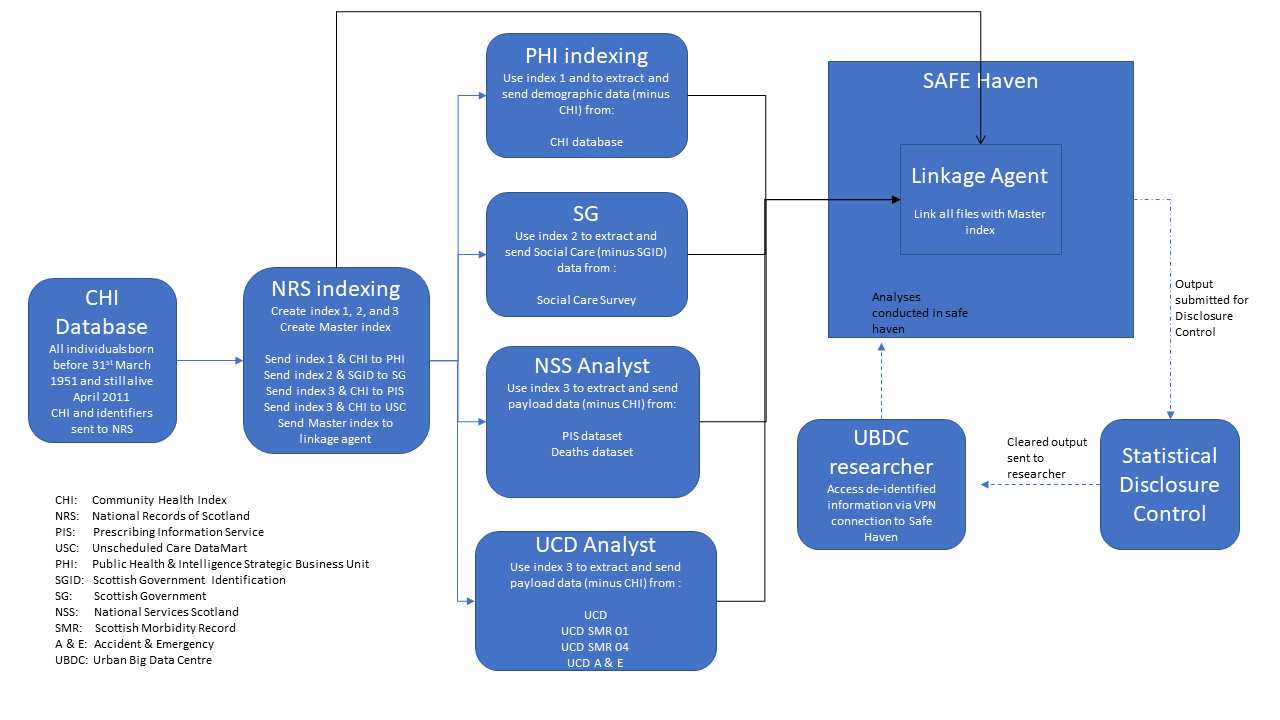
\includegraphics{figures/chapter-methods/linkage_diagram.png}
    \label{fig:methods-linkage}
\end{figure}
\end{landscape}

\FloatBarrier

\subsection{Demographic, geographic, and deaths information}\label{subsubsec:nrs-summs}

Demographic information for all eligible individuals identified from the
population spine was extracted by the Public Health and Intelligence:
Strategic Business Unit at NSS. This was joined with a flag variable
indicating if an individual was resident in a care home (from
prescribing data) in a single file which was made available in the
national safe haven. SIMD decile was assigned as per the most recent
version of the area-based measure {[}@RN238{]}.

Only month and year of birth were provided to avoid disclosure of
identifiable information. Age was calculated by flooring each
individual's \textbf{day}-of-birth to the 1st of the month-of-birth
provided and then calculating the difference between this pseudo
date-of-birth and the 31st of March in each financial year.

The number of observations, individuals, and the differing variables in
this raw demographic file are shown in table \ref{tab:demos}.

\begin{table}[h]
\centering
\caption{Demographic file data}
\label{tab:demos}
\resizebox{\textwidth}{!}{%
\begin{tabular}{@{}lll@{}}
\toprule
Number of rows & Number of individuals & Variables \\ \midrule
1,348,310 & 1,134,445 & \begin{tabular}[c]{@{}l@{}}Index, year/month of birth, year/month of death\\ Sex, Address start date, Address end date, Care home flag,\\ Previous Local Authority, Current Local Authority, \\ Current Health Board, SIMD decile\end{tabular} \\ \bottomrule
\end{tabular}%
}
\end{table}

As the table indicates, some individuals had more than one row of
information indicating multiple addresses during the study period (and
thus potential multiple values for local, authority, health board, care
home flag, and SIMD decile). Financial year time intervals were created
for using the \texttt{lubridate} software package {[}@RN522{]}. Dummy
variables were then created indicating the age, local authority of
residence, health board of residence, and SIMD decile during each
financial year (with null values where not applicable). The variables
were then gathered to long format in order to reshape the data to
include one row of data per individual per financial year. Where an
individual had multiple addresses during one financial year, the most
recent value for local authority, health board, and SIMD decile was
used. This resulted in a data frame of 7,775,410 observations pertaining
to 1,134,445 individuals.

\FloatBarrier

\subsection{Social Care Survey}\label{subsubsec:scs-summs}

Data from the Scottish Care Surveys 2010 - 2016 (including separate Home
Care Census and Self-Directed Support surveys for earlier years) were
extracted by a Scottish Government analyst and transferred to the
national safe haven in a single file. There were a number of variables
indicating the weekly hours of home care (if any) each individual
received, whether they were provided by the local authority or and
independent organisation, and whether these hours indicated the
scheduled hours of home care or the actual number of hours delivered.
There is some discrepancy between local authorities on which value
(scheduled, or actual) of home care is returned to the Scottish
Government for the SCS. Some authorities return scheduled only, others
actual hours only, and yet others return both values. The SCS reports
statistics based on the actual hours of home care delivered where
available and uses the scheduled value where it is not. This convention
was also used for the purposes of this thesis.

Many variables requested from the SCS had large amounts of missing data.
There were also coding issues with extra values present that had no
corresponding description in the provided metadata. Variables with these
issues were dropped and not included in analyses. Table
\ref{tab:scs-vars} lists the variables included and excluded after data
cleaning.

A small fraction of observations (198 pertaining to 129 individuals) had
an impossible value of weekly hours of home care greater than 168 hrs
(more than 24hr-7-day-a-week care). These records were dropped from the
dataset after being joined to other sources of data (section
\ref{subsec:join-data}).

Assessment for duplicated rows indicated 4,357 individuals had more than
one row of data for some years of data. Inspection of these additional
rows indicated a change in value for some variables (e.g.~a flag
indicating use of community alarm services positive in one row and
negative in another, or different values for client group in multiple
rows). These additional rows amounted to 1.1\% of observations in the
SCS. The exact cause of these duplications is unknown. One possible
explanation is that duplication was created when records from different
sources were joined together in advance of being sent for linkage. A
further potential cause is the duplication of records created by the
process of recycling identification numbers in some local authorities.
Given the small percentage or records this affected, individuals with
duplicated information were dropped from the dataset after being joined
to other datasets (as described in section \ref{subsec:join-data}).

\begin{table}[]
\caption{Social Care Survey file data}
\label{tab:scs-vars}
\resizebox{\textwidth}{!}{%
\begin{tabular}{@{}lllll@{}}
\toprule
Number of rows & Number of individuals & Included variables & Derived variables & Dropped variables \\ \midrule
663,809 & 227,345 & \begin{tabular}[c]{@{}l@{}}1. Index (ID)\\ 2. Living alone\\ 3. Community Alarm\\ 4. Other telecare\end{tabular} & \begin{tabular}[c]{@{}l@{}}1. Total weekly hours of home care\\ 2. Home care hours group (e.g 1-5, 6-10 etc.)\\ 3. Alarm or Telecare flag\end{tabular} & \begin{tabular}[c]{@{}l@{}}1. Client Group\\ 2. Eligibility Category\\ 3. Housing Support\\ 4. Multi Staffing\\ 5. Scheduled Hours\\ 6. Actual Hours\end{tabular} \\ \bottomrule
\end{tabular}%
}
\end{table}

\FloatBarrier

\subsection{Prescribing Information Service}\label{subsec:pis-summs}

Community prescribing information for all individuals in the cohort were
extracted from the Prescribing Information System (PIS) by analysts from
ISD. For each quarter of the study period (Quarter 1 2010/11 to Quarter
4 2015/16) a list of medicines prescribed to each individual was
extracted and transferred in one file to the national safe haven. This
file contained 134,377,877 observations of four variables: The financial
year and quarter, the BNF subsection code, The approved name of the
medicine, and a count of how many times the medicine was prescribed in
the quarter. Coding errors were found in 138,973 observations (wrong
number of digits in the BNF subsection or characters found in the count
variable) and these were dropped from analysis.

The count of medicines was based on the BNF classes included in a count
of polypharmacy by Guthrie et al {[}-@RN274{]}. The additional material
provided on-line with this paper included a table of included drugs.
This table was amended to remove BNF subsections 3.9.1, 3.9.2, and 13.9.
The latter section includes different forms of shampoos whilst the
former 2 sections include preparations for coughs. These were not deemed
necessary to be included in overall counts. Two BNF subsections not
included in the Guthrie et al table were deemed important to include as
testing revealed large numbers of prescriptions included medicines from
these sections would have been omitted otherwise. These sections were
2.2.4 (Potassium sparing diuretics with other diuretics) and 2.2.8.
(Diuretics with potassium). In total, 198 medicines listed in the BNF
were not included and rows with these medicines were removed from the
PIS file. A full list of these medicines is shown in Appendix G. Table
\ref{tab:dropped-meds} shows the cleaning process.

\begin{table}[h]
\centering
\caption{Data cleaning of PIS file}
\label{tab:dropped-meds}
\begin{tabular}{@{}lll@{}}
\toprule
Reasons & Records dropped & Records remaining \\ \midrule
Initial data file & N/A & 134,377,877 \\
Coding errors & 138,973 & 134,238,904 \\
Did not appear in Guthrie et al (2012) table & 1,427,643 & 132,811,261 \\
BNF sections 3.9.1, 3.9.2, \& 13.9 & 645,900 & 132,165,361 \\ \bottomrule
\end{tabular}
\end{table}

A summary measure for each individual was created counting the total
number of repeat medicines prescribed in each financial year. To be
eligible in the count, a medicine had to be prescribed in at least 2
quarters of each financial year. This meant one-off prescriptions, such
as antibiotics for a transient infection, were not included in the
overall count. A separate count was conducted for individuals who died
in the first quarter of each financial year (and thus unable to have
medicines prescribed in two quarters). The total number of unique
medicines prescribed in the first quarter was used for these
individuals. Each participant could thus have a maximum of 6
observations, one for each financial year. A second count was created
totalling the number of chapters of the BNF that each individual had
medicines prescribed from as a crude measure of body systems requiring
medication. Table \ref{tab:PIS-clean} shows the total observations and
variables in the cleaned PIS file.

\begin{table}[h]
\centering
\caption{Description of cleaned PIS file}
\label{tab:PIS-clean}
\begin{tabular}{@{}lll@{}}
\toprule
Number or rows & Number of individuals & Variables \\ \midrule
5,501,820 & 1,066,395 & \begin{tabular}[c]{@{}l@{}}1. Index (id)\\ 2. Financial Year\\ 3. Total medicines (n)\\ 4. Total chapters (n)\end{tabular} \\ \bottomrule
\end{tabular}
\end{table}

\FloatBarrier
\subsection{Unscheduled care measures}\label{subsec:usc-summs}

Unscheduled care information for all individuals included in the cohort
was extracted from unscheduled care data mart (UCD) by an analyst from
ISD. The raw file contained 3,772,402 observations from 845,893
individuals. Each observation related to a single continuous urgent care
pathway (CUP) as described in section \ref{subsec:source-ucd}.

In a similar fashion as with the demographics data, dummy variables were
created indicating if each observation occurred within financial years
during the study period. This enabled data to be reshaped to a long
format with individuals having one or multiple rows of data for each
financial year. To create one observation per individual per year, data
with information on each CUP was nested within a data frame as a list
column as described by Wickham \& Grolemund {[}-@RN557, ch.20{]}. With
data in this format, summary measures were derived by applying functions
to the list column utilising the \texttt{purrr} software package
{[}@RN523{]}. Derived information included counts of total USC episodes,
acute admissions to hospital, A \& E attendances, and total number of
long-term conditions identified from admissions and A \& E data. The
format of the cleaned UCD data frame is described in table
\ref{tab:USC-clean}

\begin{table}[h]
\caption{Description of cleaned USC file}
\label{tab:USC-clean}
\begin{tabular}{@{}lll@{}}
\toprule
Number of rows & Number of individuals & \multicolumn{1}{c}{Variables} \\ \midrule
1,951,755 & 845,516 & \begin{tabular}[c]{@{}l@{}}1. Index (id)\\ 2. Year\\ 3. USC episodes (n)\\ 4. Acute admissions (n)\\ 5. A \& E attendances (n)\\ 6. Long-term conditions (n)\end{tabular}\\ \bottomrule
\end{tabular}
\end{table}

Data were available beyond the study period ending 31st March 2016.
Records outside this end date were dropped when this file was joined
with the other sources of data which is described in the next section.

\FloatBarrier

\subsection{Joining sources together}\label{subsec:join-data}

\FloatBarrier

Following cleaning and formatting of each individual file, further
wrangling was completed which joined each file together in a parent data
frame to be used for analysis. This involved loading individual files in
one-by-one and joining them together using the ``full join'' function
from the R package \texttt{dplyr} {[}@RN283{]} using the unique index
number as the joining parameter. This process ensured all records were
retained, even if an index number was only present in one file.

With all study data now in one data frame, further cleaning and tidying
was required. This was an iterative process. As initial descriptive and
statistical analysis was completed, identification of errors and data
quality issues required repetition of the joining process to address
these issues. This process is now described with a summary provided in
table \ref{tab:joining}.

\begin{table}[h]
\caption{Joining files together and cleaning process}
\label{tab:joining}
\resizebox{\textwidth}{!}{%
\begin{tabular}{lrr}
\hline
 & \multicolumn{1}{l}{Number of rows} & \multicolumn{1}{c}{\begin{tabular}[c]{@{}c@{}}Total number of rows remaining\\ after join/drop\end{tabular}} \\ \hline
Cleaned demography file & 7,775,410 & 7,775,410 \\
Cleaned prescribing information file & 5,501,820 & 8,057,604 \\
Cleaned social care file & 663,809 & 8,072,233 \\
Cleaned unscheduled care file & 1,951,755 & 8,094,256 \\
After age and death tidying process &  & 8,115,549 \\
Duplicates & 14,809 & 8,100,740 \\
Missing data for Local Authority & 7,435 & 8,056,329 \\
Age \textless{}65 OR Clackmannanshire OR data for 2017/18 & 1,832,443 & 6,223,886 \\
Home care hours \textgreater{}168 per week & 198 & 6,223,688 \\
Died before 65 years of age & 8808 & 6,214,880 \\
Implausible SIMD value & 23 & 6,214,857 \\
Data from years 2010/11 OR 2016/17 & 1,695,602 & 4,519,255 \\ \hline
\end{tabular}%
}
\end{table}

Once all files had been joined together the parent dataframe contained
8,094,256 observations. As there were discrepancies over time periods
for which data was provided in different files, the calculation of age
from the demographic file was not always present for all years of data
(e.g.~where demographic data was returned for the years 2015-2018 and
PIS data was available from 2011-2018). To ovecome this, age was
recalculated from the pseudo date-of-birth (described in section
\ref{subsubsec:nrs-summs}) for all financial years. Where an indivudal
died during a financial year, the age variable was left empty which
required additional rows to be added in some cases.

As described in section \ref{subsubsec:scs-summs}, Approximately 4000
individuals had duplicated social care information for some years of
data. These rows, and other duplicates created by the cleaning process
involving age and date-of-death variables, were then dropped.

For the same reasons that age values were not shown in every year of
data, values for sex, local authority of residence, health board, and
SIMD decile were missing from 50,349 of observations (1.11\% of the
final cleaned data frame). These observations were filled by carrying
the last observation forward. Whilst this would not have affected values
for sex, potential error could have be introduced to the other
variables. Given the small percentage of affected observations this was
deemed acceptable. Despite this, there were still 7,435 records with
missing values for local authority. Cross referencing these indiviudal
rows with the raw demographics data file revealed the values for local
authority in these observations were true missing data (not created by
data manipulation). Given the small proportion of records these
represented they were dropped from the data frame.

A further 1,832,443 observations were then removed from the data frame.
These observations were for years of data where indivudals were either:
(a) under 65 years of age (the cohort comprised indivudals over 65 or
\emph{turning} 65 during the study period), (b) resident in the
Clackmannanshire local authority area (linkage rates of the social care
survey to the indexing spine were too low to be reliable in this
council. (See section \ref{sec:linkage} for details), or (c) contained
unscheduled care data for financial year 2017/18 which was well beyond
the study period.

Exploratory data analysis revealed three data quality issues that
required further observartions to be dropped from the data frame.
Firstly, as described in section \ref{subsubsec:scs-summs}, 168
observations contained implausible values for weekly hours of home care
(\textgreater{}168 hrs). These had not been removed as whilst cleaning
the social care file so were dropped here. Secondly, calculating average
age for each individual revealed 8,808 observations with a null value.
Further inspection of these observations identified each individual had
only one observation and had died before their 65th birthday. The
inclusion criteria for the cohort stated individuals should be ``born
before 31st March 1951 and alive during the study period 1st April 2011
to 31st March 2016''. This meant, for example, an indivudal born on
Christmas day 1949 and dying at age 64 on Christmas day 2013 was
extracted as part of the cohort data. These observations were also
dropped from the parent data frame. Finally, 23 rows of data were found
to have implausible values for SIMD decile. These observations were from
individuals living in either the Shetland Islands or Na h-Eileanan Siar
which only have datazones in 5 deciles making values outwith these
deciles impossible.

Whilst the study period had been defined as 1st April 2011 to 31st March
2016 some data files contained observations outwith this period. These
1,695,602 observations were maintained for exploratory analysis but were
dropped for final analysis. Thus, the final parent dataframe used for
all reported analyses contained 4,519,255 observations.

Derived grouping variables were created for age group (5 year bands),
repeat medicines group (4 groups of similar size: 0-2, 3-5, 6-8, and
over 9 repeat medicines), and linkage group (grouping councils that had
linkage rates (described in section \ref{sec:linkage} within 4\% of each
other e.g.~96-99.9\%, 92-95.9\% etc.)

\FloatBarrier

\section{Statistical methods}\label{sec:methods-stats}

\subsection{Research question 1}\label{stats-rq1}

To address the question of how multimorbidity plus sociodemographic and
geographic factors influence the utilisation of social care, logistic
regression models were fitted seperately to each financial year of data.
The dependent variable in these models was receipt of any form of social
care, measured by presence or not in the social care survey. Independent
variables and interaction terms were added incrementally to assess
impact on model fit which was measured by McFadden's pseudo \(R^2\)
{[}@RN561{]} calculated by the formula

\[R^{2}_{McFadden} = 1 - \frac {ln(LM_{1})}{ln(LM_{0})} \] Where:

\(ln(LM_{1})\) = log likelihood of the fitted model and:\newline
\(ln(LM_{0})\) = log likelihood of the null model (with intercept only
as a predictor).

McFadden's \(R^2\) values are not analagous with \(R^2\) values
calculated from linear models. Instead, values of 0.2 - 0.4 represent an
excellent model fit {[}@RN562,p35; @RN560,p55{]}.

The final models included sex, age group, repeat medicines group, SIMD
decile of residence, and local authority of residence as independent
variables. Interaction terms were fitted between: sex \& age group, age
group \& repeat medicines group, SIMD decile \& repeat medicines group,
and SIMD decile \& local authority of residence. Exploratory models had
revealed a linear effect of SIMD decile on receipt of social care thus,
given the complexity of interaction terms and subsequent computational
requirement, SIMD was fitted as a continuous term in the final models.

All other independent variables were categorical in nature with a number
of interaction terms fitted which can make misinterpretation of
logisitic regression models more likely {[}@RN563; @RN564; @RN565{]}.
Therefore, estimated effects are reported as average partial effects
(APEs) described by Mood {[}-@RN563, p75{]} with the formula

\[\frac{1}{n}\sum_{i = 1}^n\beta_{x_1}f(\beta_{x_i)\] where
\(\beta_{x_1}\) is the log odds-ratio for variable \(x_{1}\),
\(\beta_{x_i}\) is the value of the logit for the \(i\)-th observation,
and \(f(\beta_{x_i})\) is the probability distribution function of the
logistic distribution with regard to \(\beta_{x_i}\). The effect
estimate describes the average marginal effect (AME) at a specific value
of \(x_1\). Williams {[}-@RN566,p325{]} provides an intuitive example of
how APEs are calculated and interpreted which is adapted for the current
model with the ``sex'' variable here:-

\begin{itemize}
\tightlist
\item
  Go to the first case. Treat that observation as if they were male
  regardless of actual sex. Leave other values of independent variables
  at their observed value. Compute the probability of receiving social
  care with the fitted model (including interaction terms).\\
\item
  Repeat but change the value of sex to female
\item
  The difference in the two probabilities is the partial (marginal)
  effect for that case.
\item
  Repeat for every observation in the data.
\item
  Compute the average of all the partial effects. This gives the APE for
  being female.
\end{itemize}

Mood {[}@RN563{]}

\subsection{Research question 2}\label{stats-rq2}

\section{Timeline}\label{sec:timeline}

Describe timeline of approvals process - major hurdles and barriers.
\textbf{Maybe in methods??}

\section{Conclusion}\label{sec:data-conclusion}

Brief summary of chapter here


\end{document}
